\section{Square Deal}
\label{squaredeal}
\href{https://open.kattis.com/problems/squaredeal}{View on Kattis}\\
\textbf{Tags:} Brute Force, Geometry\\
\subsection{Problem Description}
Given the width and height of 3 rectangles, can you arrange the rectangles to
form a square?
\subsection{Algorithm}
Because there are exactly 3 rectangles, there are only 2 cases that we need to
consider:
\begin{itemize}
  \item All rectangles can be stacked in a line together (Figure
    \ref{squaredeal:case-1}).
  \item 2 rectangles are stacked together. The other will lie across them
  (Figure \ref{squaredeal:case-2}).
\end{itemize}

\begin{figure}[h!]
  \centering
  \begin{minipage}{0.45\textwidth}
    \centering
    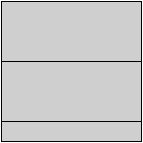
\includegraphics[width=0.9\textwidth]{Images/squaredeal-case1.png}
    \caption{Case 1}
    \label{squaredeal:case-1}
  \end{minipage}\hfill
  \begin{minipage}{0.45\textwidth}
    \centering
    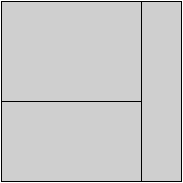
\includegraphics[width=0.9\textwidth]{Images/squaredeal-case2.png}
    \caption{Case 2}
    \label{squaredeal:case-2}
  \end{minipage}
\end{figure}

We can brute force this quite easily. All we need to do is examine all
8 combinations of vertical/horizontal rotations, and then check both cases for
each combination. The first case is one check, and for the second case, we will
need to try all 3 rectangles as the one that isn't stacked with the others.\\

\hfill\break
\textbf{Time Complexity:} $\mathcal{O}(2^{N} \cdot N)$\\
\textbf{Space Complexity:} $\mathcal{O}(N)$\\
Where $N$ is the number of rectangles (3).
\pagebreak
\subsection{Implementation}
\lstinputlisting[
  lastline=47,
  language=Java
]{Solutions/SquareDeal.java}
\pagebreak
\lstinputlisting[
  firstline=49,
  language=Java
]{Solutions/SquareDeal.java}
\pagebreak
